\documentclass{standalone}
\usepackage{tikz}
\usetikzlibrary{calc}
\begin{document}

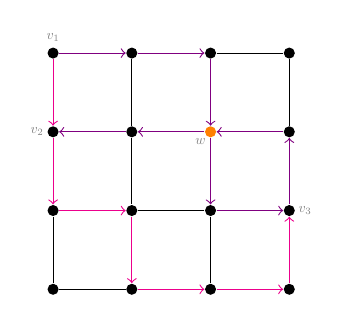
\begin{tikzpicture}[
  every node/.style={circle, fill=black, inner sep=1pt, minimum size=4pt}
]


  \node[label={[gray, scale=0.5]above:$v_1$}] (a1) at (5,3) {};
  \node (b1) at (6,3) {};
  \node (c1) at (7,3) {};
  \node (d1) at (8,3) {};
  \node[label={[gray, scale=0.5]left:$v_2$}] (e1) at (5,2) {};
  \node (f1) at (6,2) {};
  \node[label={[gray, scale=0.5]below left:$w$}] (g1) at (7,2) [fill=orange]{};
  \node (h1) at (8,2) {};
  \node (i1) at (5,1) {};
  \node (j1) at (6,1) {};
  \node (k1) at (7,1) {};
  \node (l1)[label={[gray, scale=0.5]right:$v_3$}] at (8,1) {};
  \node (m1) at (5,0) {};
  \node (n1) at (6,0) {};
  \node (o1) at (7,0) {};
  \node (p1) at (8,0) {};




  \draw (c1) edge[-](d1);
  \draw (d1) edge[-](h1);
  \draw (k1) edge[-](j1);
  \draw (m1) edge[-](n1);
  \draw (m1) edge[-](i1);
  \draw (f1) edge[-](j1);
  \draw (b1) edge[-](f1);
  \draw (k1) edge[-](o1);
  \draw (a1) edge[->, violet](b1);
  \draw (b1) edge[->, violet](c1);
  \draw (c1) edge[->, violet](g1);
  \draw (g1) edge[->, violet](k1);
  \draw (k1) edge[->, violet](l1);
  \draw (l1) edge[->, violet](h1);
  \draw (h1) edge[->, violet](g1);
  \draw (g1) edge[->, violet](f1);
  \draw (f1) edge[->, violet](e1);

  \draw (a1) edge[->, magenta](e1);
  \draw (e1) edge[->, magenta](i1);
  \draw (i1) edge[->, magenta](j1);
  \draw (j1) edge[->, magenta](n1);
  \draw (n1) edge[->, magenta](o1);
  \draw (o1) edge[->, magenta](p1);
  \draw (p1) edge[->, magenta](l1);

\end{tikzpicture}

\end{document}
